\section{高效的聚合索引算法}
\label{sec5:solution}

首先,我们提出了一个叫做区间森林法(Range Forest Solution,RFS)的算法来维护每条边上的数据点,以支持高效的聚合向量动态查询。

\subsection{区间森林法}
\label{subsec:RFS}

	区间树~\cite{de2000computational} 是一种高效的树形数据结构,它以层次化的方式维护数据点,其中每一个树节点都代表了若干数据点的聚合集。

	首先,所有的数据点会按照他们在边上的相对位置排序(例如根据$d(v_c, p_i)$排序),并且所有数据点都会被存入根节点中。接着,每个节点会被递归地分成两个子节点,每个节点存放一半数据点,直到只剩下一个数据点为止。具体来说,假设树节点 $u$ 存放了数据点$\{o_l,...,o_r\}$,那么它的两个子节点$lc(u)$ 和 $rc(u)$会分别存放$\{o_l,...,o_{\lfloor (l + r) / 2 \rfloor}\}$ 和 $\{o_{\lfloor (l + r) / 2 \rfloor + 1},...,o_r\}$。这样,每个节点都维护了一个区间内的节点,即 $R(u) = [d(v_c, o_l), d(v_c, o_r)]$。
	
	\begin{figure}[h!]\centering
	\scalebox{0.5}[0.5]{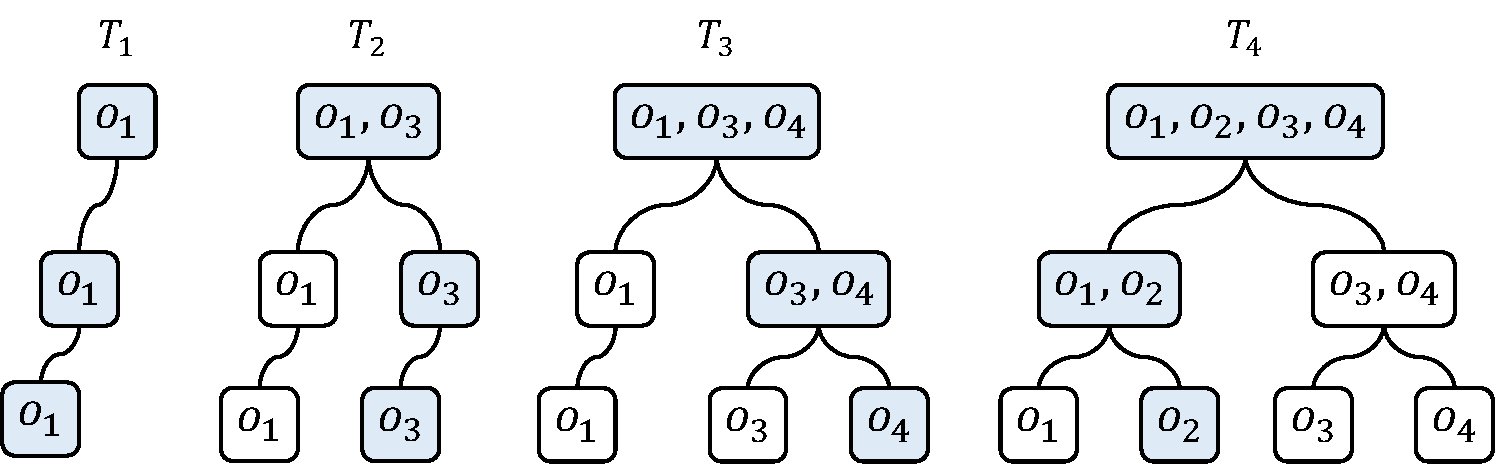
\includegraphics{./figures/RFS_1.pdf}}
	\caption{一个包含四个数据点的范围森林的例子,时间次序为$\{o_1, o_3, o_4, o_2\}$。}
	\label{fig:RFS1}
	\end{figure}
		

	图~\ref{fig:RFS1}中的 $T_4$ 就是一个区间树的例子,其中$o_1, o_2, o_3, o_4$四个数据点在边上位置依次从左往右。根节点包含四个数据点,每个树节点都继承了父节点中的一半数据点。

	仅仅一棵区间树只能维护空间信息,为了加入时间信息,我们可以将数据点动态插入,并可持久化地记录所有中间状态,构成一系列区间树,也就是一个区间森林。图~\ref{fig:RFS1}是一个区间森林地例子,假设四个数据点的时间顺序为$o_1, o_3, o_4, o_2$,每次插入都会在原有的区间树上加入一个数据点,构成一棵新的区间树,其中更新的节点用蓝色表示,白色节点表示不变。注意,树节点所维护的区间$R(u)$是根据最后结果(即 $T_4$ )决定且不会变化的,即使其中的数据点还未被插入。

\subsection{区间森林上的查询}

	区间森林上的查询包含两个步骤,即\textbf{生成}和\textbf{探查}。

	\textbf{生成:} 通过将两棵区间树“相减”,可以得到一棵新的区间树,且其中包含这个时间段内的所有数据点。图~\ref{fig:RFS2}给出了一个包含数据点 $o_3$ 和 $o_4$ 的例子。因此,对于任意一个时间窗口,我们都可以快速获取该时间窗口内所有数据点构成的区间树。
	
\begin{figure}[h!]\centering
	\scalebox{0.5}[0.5]{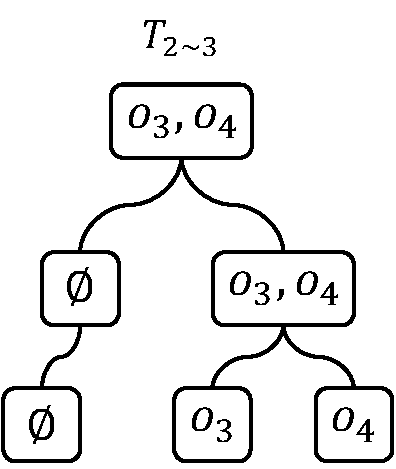
\includegraphics{./figures/RFS_2.pdf}}
	\caption{一个区间森林查询的例子。通过查询时间窗口,我们可以生成仅包含两个数据点$o_3$ 和 $o_4$的区间树。}
	\label{fig:RFS2}
\end{figure}

	\textbf{探查:} 在生成了特定的区间树后,时间维度上的查询就已经结束,接下来只需要将空间查询中的边界条件代入即可。在第三章中已经给出了 $v_c$ 侧的两个边界条件:(1)数据点的位置不能超过带宽范围 $b_s$ 和(2)数据点的位置必须距离 $v_c$ 更近,即:
	\begin{equation*}
	\begin{aligned}
		d(v_c, p_i) &\le b_s - d(q, v_c) \\
		d(v_c, p_i) &\le \frac{-d(q, v_c) + d(q, v_d) + d(v_c, v_d)}{2}
	\end{aligned}
	\end{equation*}
	
	另 $R = [0, \min(b_s - d(q, v_c), \frac{-d(q, v_c) + d(q, v_d) + d(v_c, v_d)}{2})]$ 表示查询的区间,我们需要这个区间内所有的数据点,即$d(v_c, p_i) \in R$,及它们所对应的聚合集。这个步骤可以通过在区间树上递归查询解决,具体步骤如算法~\ref{algo:RFQ}所示。假设查询的时间范围是 $[T_l, T_r]$,那么我们需要用 $T_r$ 时刻的区间树减去 $T_{l-1}$ 时刻的区间树。注意我们并不需要真的构造这一棵树,而是直接在两棵已有的区间树上遍历。我们用两个变量$u_l$ 和 $u_r$记录这个遍历过程,初始值为两个根节点。每次递归时有三种可能:
	\begin{itemize}
		\item 如果 $R(u_r) \cap R = \varnothing$~(第4行),说明该区间树节点的所有数据点都不包含在查询的区间内,直接返回零向量;
		\item 如果$R(u_r) \subseteq R$~(第6行),说明所有的数据点都包含在查询的区间内,可以直接返回这些数据点对应的聚合向量,即$\mathbf{A}(u_r) - \mathbf{A}(u_l)$,这里利用到了聚合向量的计算可逆性;
		\item 否则,需要在两个子节点中进一步查询(第8行)。
	\end{itemize}

	\begin{algorithm}[h]
		\caption{区间森林查询}
		\label{algo:RFQ}
		\DontPrintSemicolon
		\KwIn{the temporal query range $[T_l, T_r]$ \\ \hspace{2.75em} the spatial query range $R$}
		\KwOut{the aggregated vector $\mathbf{A}$}

		$u_l \leftarrow root(T_{l-1}), u_r \leftarrow root(T_r)$
		
		\Return{$DualDetect(u_l, u_r)$}
		
		\SetKwFunction{DQ}{DualDetect}
		\SetKwProg{Fn}{Function}{:}{}
		\Fn{\DQ($u_l, u_r$)}{
		
		\uIf{$R(u_r) \cap R = \varnothing$}{
			\Return{$\mathbf{0}$}
		}
		\ElseIf{$R(u_r) \subseteq R$}{
			\Return{$\mathbf{A}(u_r) - \mathbf{A}(u_l)$}
		}
		\Else{
			\Return{
				$DualDetect(lc(u_l), lc(u_r)) + DualDetect(rc(u_l), rc(u_r))$
			}
		}
		}
	\end{algorithm}

区间森林的查询非常高效,达到了和传统的二分查询一样的时间复杂度:

\begin{lemma}
	给定一个在边 $e$ 上的查询,算法~\ref{algo:RFQ} 需要 $O(\log{n_e})$ 的时间来获取聚合向量,其中 $n_e$ 表示边 $e$ 上的数据点个数。
\end{lemma}

\begin{proof}
	将连续的时间窗口映射到实际的查询范围$[T_l, T_r]$需要使用二分查询,花费$O(\log{n_e})$。在\textit{DualDetect}函数中,每个节点只有三种情况:不覆盖(第4行),全覆盖(第6行),和部分覆盖(第8行)。对于部分覆盖的节点,它的子节点同样有两种情况:如果左子节点是部分覆盖,那么右子节点不覆盖;如果右子节点是部分覆盖,那么左子节点全覆盖。因此,在该递归操作所对应的区间树中,部分覆盖的节点数量只会减少不会增加,即每一层最多只有一个,所以每一层中最多只会有两个节点会被访问到。因此,查询时间复杂度为区间树的高度。此外,由于区间树是平衡的,所以树的高度为$\lceil\log{n_e}\rceil$,时间复杂度为$O(\log{n_e})$。
\end{proof}

\subsection{区间森林的构造}

	如果我们直接如图~\ref{fig:RFS1}所示构造完整的区间森林,虽然查询速度和二分查询类似,但索引会占用大量的内存空间。注意到相邻的两棵区间树存在高度相似的结构(白色节点),只有$O(\log n_e)$个被插入的树节点存在不同。因此,我们可以只记录这些更新的节点,而另外不变的节点可以直接链接到原区间树上。如图~\ref{fig:RFS3}所示,这种共享结构只会改变底层的数据引用,对节点之间的逻辑关系不会有任何影响。因此,算法~\ref{algo:RFQ}无需任何修改。
	
	\begin{figure}[h!]\centering
		\scalebox{0.5}[0.5]{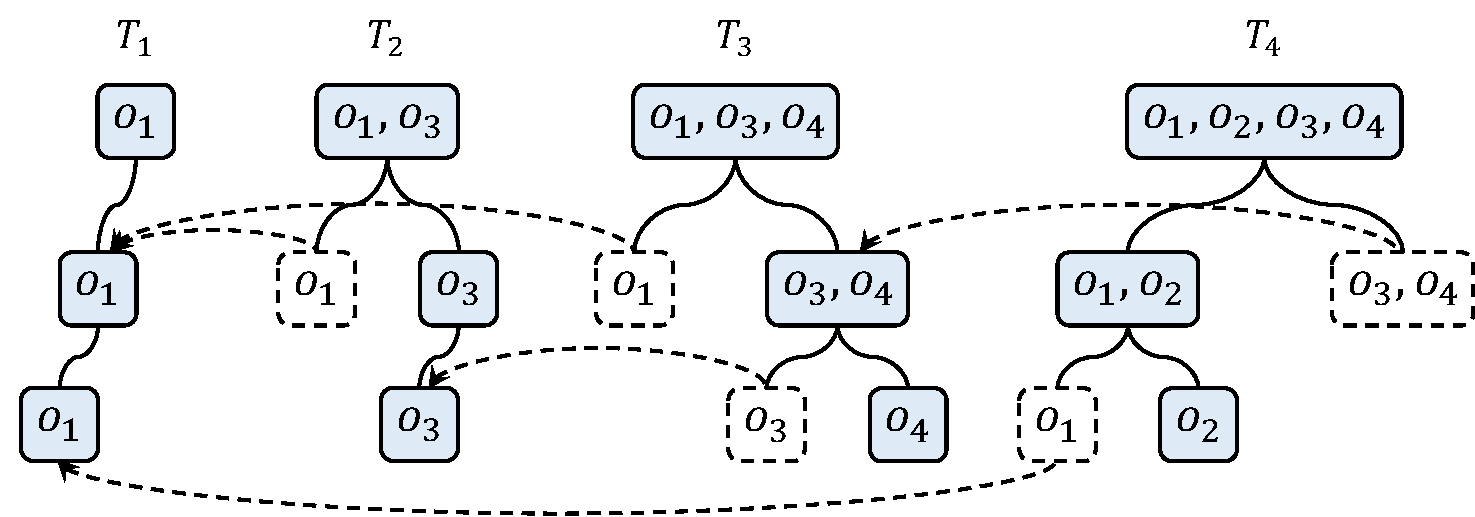
\includegraphics{./figures/RFS_3.pdf}}
		\caption{共享内存版本的区间森林。只有被更新的节点(用蓝色标记)是实际存在的,其他没有修改的节点会被链接到前面的区间树节点上。}
		\label{fig:RFS3}
	\end{figure}

	算法~\ref{algo:RFC} 描述了优化版本的区间森林的构造流程。在第2-4行,不断有数据点按照时间顺序依次插入最新的区间树中。在每次构造中,树节点会被动态创建(第6行)并更新聚合向量(第7行)。如果数据点$o_i$将被分配到左子节点$lc(u_r)$,即$d(v_c, p_i) \in R(lc(u_l))$,那么不变的右子节点会被链接到原区间树的节点$rc(u_l)$上,并且向左边继续递归;另一侧的更新操作同理。
	
	\begin{algorithm}[h]
		\caption{区间森林构造}
		\label{algo:RFC}
		\DontPrintSemicolon
		\KwIn{event set $\{o_i\}$ on the edge $e$}
		\KwOut{range forest $T_i$}
	
		sort $\{o_i\}$ by time $t_i$
		
		\For{$i \in [1, n_e]$}{
			$u_l \leftarrow root(T_{i-1})$
		
			$root(T_i) \leftarrow DualConstruct(u_l, o_i)$
		}
			
		\SetKwFunction{DC}{DualConstruct}
		\SetKwProg{Fn}{Function}{:}{}
		\Fn{\DC($u_l, o_i$)}{
		
		create a new tree node $u_r$
		
		$\mathbf{A}(u_r) \leftarrow \mathbf{A}(u_l) + \mathbf{A}(o_i)$
			 
		\uIf{$d(v_c, p_i) \in R(lc(u_r))$}{
			link $rc(u_r)$ to $rc(u_l)$
			
			$lc(u_r) \leftarrow DualConstruct(lc(u_l), o_i)$
		}
		\Else{
			link $lc(u_r)$ to $lc(u_l)$
			
			$rc(u_r) \leftarrow DualConstruct(rc(u_l), o_i)$
		}
		
		\Return{$u_r$}
		}
			
	\end{algorithm}

经过优化后的区间森林构造时间复杂度和排序操作一样,因此可以认为是最够高效的:

\begin{lemma}
	对于一条边 $e$,算法~\ref{algo:RFC} 可以在$O(n_e\log{n_e})$的时间和空间复杂度内构造一个区间森林,其中 $n_e$ 表示边 $e$ 上的数据点个数。
\end{lemma}

\begin{proof}
	区间森林包含 $n_e$ 棵区间树,对于一棵区间树的构造,每次只会往一个方向递归,因此需要递归$\left\lceil\log{n_e}\right\rceil$次,每次操作都是常数复杂度,因此每棵区间树的构造时间均为 $O(\log{n_e})$,总时间复杂度为$O(n_e\log{n_e})$。由于每个树节点都是动态创建的,每次递归只会创建一个节点,因此总空间复杂度也为$O(n_e\log{n_e})$。
\end{proof}

使用和引理~\ref{lemma:ADA}相同的技巧,我们可以计算得到RFS算法的总时间复杂度和空间复杂度。

\begin{lemma}
	\label{lemma:RFS_1}
	RFS算法的查询部分时间复杂度为$O(\vert E \vert (T_{sp} + L \cdot \log\frac{N}{\vert E \vert}))$,索引构造部分的时间复杂度在最坏情况下是$O(N \cdot \log{N})$。空间复杂度在最坏情况下是$O(N \cdot \log{N})$。
\end{lemma}
\begin{proof}
	对于查询部分,RFS算法和ADA算法的时间复杂度是相同的,即在边 $e$ 需要$\log{n_e}$的时间复杂度查询,因此使用相同的后续分析方式可以得到时间复杂度为$O(\vert E \vert (T_{sp} + L \cdot \log\frac{N}{\vert E \vert}))$。

	对于索引构造部分,每条边 $e$ 上的索引是一个树状结构,因此需要$O(n_e \log{n_e})$的时间构造,注意到:
	\begin{equation*}
		\sum_{e \in E} n_e \log{n_e} \le \sum_{e \in E} n_e \log N = N \log N
	\end{equation*}
	因此最坏情况下的构造时间复杂度为 $O(N \log N)$,当且仅当所有的数据点集中在同一条边上时成立。

	事实上,由于查询部分和索引构造部分的最坏情况是完全矛盾的(均匀分布或集中分布),这就导致具体的时间复杂度很难量化。另一方面,即使分布不集中,对于索引构造的时间复杂度的影响也只会体现在更小的 $\log N$ 中,不会影响前面的主要变量 $N$。

	对于空间复杂度来说,主要开销是区间森林的索引大小,这部分和索引构造的时间复杂度相同,即最坏情况下为 $N \log N$。
\end{proof}



	

%\clearpage









%\section{Solution1}
%\label{sec:solution1}
%
%Paragraph 1: what is the general idea of the solution1? Greedy based? DP? Generally introduce solution1.
%
%\section{some properties}
%Do you have any properties about the problem to use for developing the algorithm? Show them in this section with lemmas. 
%
%Or you need define some special values to ease your algorithm description, do it here!
%
%
%You may need to write some equations. Here I show some example equations styles.
%
%1. Multiple Equations with numbering:
%
%\begin{eqnarray}
%A &=& B \label{eq:equation1}\\
%B &=& C.\label{eq:equation2}
%\end{eqnarray}
%
%2. Single equation with numbering:
%
%\begin{equation}
%A = B \label{eq:equation3}
%\end{equation}
%
%3. Simple equation without numbering:
%$$A = B$$
%
%4. Align equations:
%\begin{eqnarray}
%&& function(A) \notag\\
%&=& A^3 +  A^2 + A^1\label{eq:equation4}
%\end{eqnarray}
%
%5. Equation with more than one conditions:
%
%\begin{equation}
%A=\left\{
%\begin{array}{ll}
%A + 1, & A \neq 0 \\
%A, & A = 0
%\end{array}
%\right. \label{eq:equation5}
%\end{equation}
%
%6. Linear Programming:
%
%\begin{alignat}{2}
%& \text{max}&  & \sum\lambda_{ik}\cdot x_{ik}\\
%& \text{s.t.}&    \quad & 
%\begin{aligned}[t]
%&d(u_i, v)\cdot x_{ik} \leq r,    &&i =1, \dots, m; k = 1, \dots, q,\\
%&\sum_{k=1}^{q} x_{ik} \leq 1,					 &&i =1, \dots, m,
%\end{aligned}\notag
%\end{alignat}
%
%\section{proposed algorithm}
%
%Your algorithm needs an interesting name! Stop simply calling it ``the Greedy algorithm'' or ``the Dynamic Programming Based Algorithm''! Do not use these boring names, please!
%
%Introduce the details of your algorithms with natural language. Below is an example of  pseudocode.
%
%
%\begin{algorithm}[t]
%	\DontPrintSemicolon
%	\KwIn{A set $C$ of $n$ workers, and a set $R$ of $m$ riders}
%	\KwOut{A set of updated scheduling sequences $S$}
%	\ForEach{$r_i \in R$}{
%		retrieve a list $C_i$ of workers that are valid to $r_i$\;
%	}
%	
%	
%	\While{$C_i \neq \emptyset$}{
%		
%		\uIf{rider $r_i$ can be arranged in $c_j$}{
%			do if.\;
%			\textbf{break}\;
%		}
%		\ElseIf{$r_i$ can replace rider $r'_i$ of $c_j$}{
%			do else.\;
%			\textbf{break}\;
%		}
%	}
%	
%		
%	
%
%	\Do{condition}{Eample of do-while-loop}
%	
%	\Return{$\mathbb{S}$}\;
%	\caption{ExampleAlgorithm}
%	\label{algo:example_algorithm}
%\end{algorithm}
%
%\section{theory analyses}
%
%Analyze the approximation ratios, competitive ratios, time complexities here.
%
